\documentclass[12pt]{article} % For LaTeX2e
\usepackage{nips11submit_e,times}
\usepackage{graphicx}
%\documentstyle[nips10submit_09,times,art10]{article} % For LaTeX 2.09

\usepackage{amsmath, amsthm, amssymb}
\usepackage{graphicx}
\usepackage{hyperref}

\newtheorem{prob}{Problem}
\newtheorem*{prop}{Proposition}
\newtheorem*{obs}{Observation}
\newtheorem*{lemma}{Lemma}
\newtheorem*{defn}{Definition}
\newtheorem*{example}{Example}
\newtheorem*{theorem}{Theorem}
\newtheorem*{cor}{Corollary}
\newtheorem*{claim}{Claim}

\newcommand{\brk}[1]{\{#1\}}
\newcommand{\res}{\text{res}}
\newcommand{\dt}{\; \text{d}}
\newcommand{\sq}{\sqrt}
\newcommand{\C}{\mathbb{C}}
\newcommand{\D}{\mathbb{D}}
\newcommand{\R}{\mathbb{R}}
\newcommand{\Q}{\mathbb{Q}}
\newcommand{\N}{\mathbb{N}}
\newcommand{\Z}{\mathbb{Z}}
\newcommand{\sm}{\setminus}
\newcommand{\F}{\mathbb{F}}
\newcommand{\GF}{\text{GF}}
\newcommand{\RS}{\text{RS}}
\newcommand{\lr}[1]{\left (#1 \right )}
\newcommand{\abs}[1]{\left | #1 \right |}
\newcommand{\floor}[1]{\lfloor #1 \rfloor}
\newcommand{\length}{\text{length}}


\title{Machine Learning Toolbox for Feature Extraction and Inference}
\author{Yo Sup ``Joseph'' Moon, Dana Modzelewski, William Chambers, Claudia Friedsam}

\newcommand{\fix}{\marginpar{FIX}}
\newcommand{\new}{\marginpar{NEW}}

\nipsfinalcopy % Uncomment for camera-ready version

\begin{document}
\maketitle


\begin{center}
CS51 Final Project April 8\textsuperscript{th}, 2012 Draft \\
Due 11:59PM, April 8\textsuperscript{th}, 2012.  
\end{center}

\begin{center}
Handwriting Recognition Toolbox Beta 0.1.0.
\end{center}

\section{Brief Overview}
 
We want to implement two different methods for unsupervised learning with the goal to extract information from high dimensional data. The algorithms we chose are principal component analysis and k-means clustering.
We want to implement the basic algorithms, test and compare them on a set of handwriting data and investigate their performance. 
We plan to address the limitations we identified by extending the algorithms with straightforward solutions like e.g. heuristics or optimization methods.  

\section{Feature}
\begin{enumerate}

	\item K-means 
	
	\emph{Fundamental Features:} 
		\begin{itemize}
			\item K-means algorithm
			\item Test functions
			\item Evaluation methods to examine performance 
		\end{itemize}
	\emph{Possible Extensions:}
		\begin{itemize}
			\item Heuristic or genetic algorithm for optimization
			\item Explore variations of k-means, e.g. density based k-		means, soft k-means 
		\end{itemize}
	\item Principal Component Analysis (PCA)\\
	\emph{Fundamental Features:}
		\begin{itemize}
			\item PCA algorithm
			\item Eigenvector Finding: can we find suitable time-efficient 			algorithm that suits our needs?  
			\item Test functions: sanity check on small-dimensional data. Test robustness of feature extraction: how much of the ``useful'' features of the data preserved?  
		\end{itemize}

	\item Common Features: \\
		\emph{Fundamental Features:}
		\begin{itemize}
			\item Method to load and prepare data to be used 
			\item GUI to load data, pick the method, adjust input parameters, visualize results and performance for both methods 
			\item Testing performance of model: k-fold cross validation, logistic regression 
			\item Testing performance for the k-means and PCA algorithms 
			\item Testing performance for handwriting data recognition 
		\end{itemize}

\end{enumerate}

\begin{center}
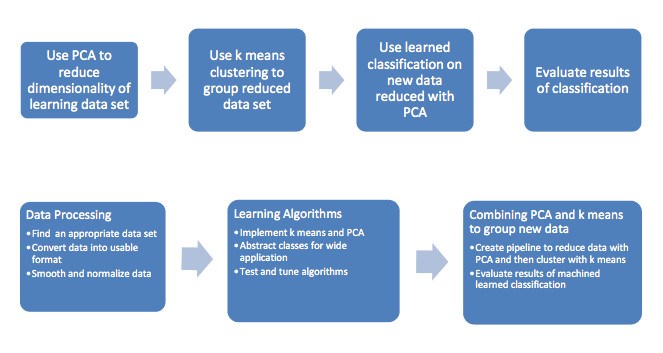
\includegraphics[width=125mm]{flowchart.png}
\end{center}


\section{Code}

\subsection{Read Data Module}
\emph{Functions:}
\begin{itemize}
	\item Read file into array 
	\item Perform data clean up (remove outliers, smoothing, etc)
	\item Export Data 
\end{itemize}

\emph{Exceptions:}
\begin{itemize}
	\item Can't read/find file
	\item File contains ill-defined data 
	\item Cleanup failed
	\item Can't write file 
\end{itemize}
 
\begin{center}
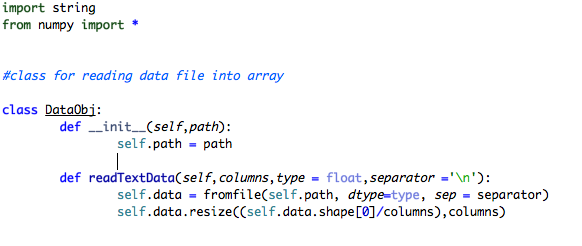
\includegraphics[width=\textwidth]{claudia4.png}
\end{center}

\subsection{K-means}
\emph{K-means Functions:}
\begin{itemize}
	\item Initialize Clusters
	\item Get centroids of partitioned data 
	\item Calculate distances of points to centroids 
	\item Reassign points to closest clusters 
	\item Export data 
\end{itemize}
\emph{Exceptions:}
\begin{itemize}
	\item Number of clusters too big 
	\item Empty clusters 
	\item Can't write file 
\end{itemize}


\begin{center}
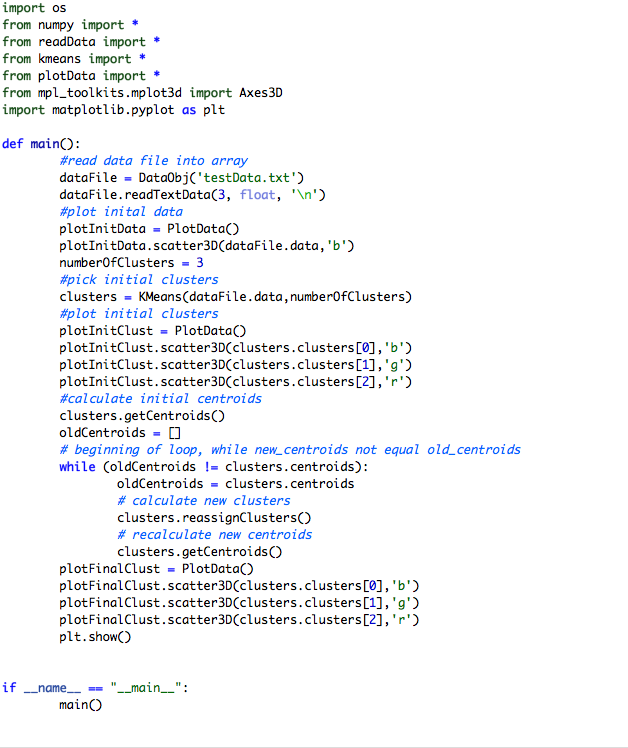
\includegraphics[width=\textwidth]{claudia2.png}
\end{center}

\begin{center}
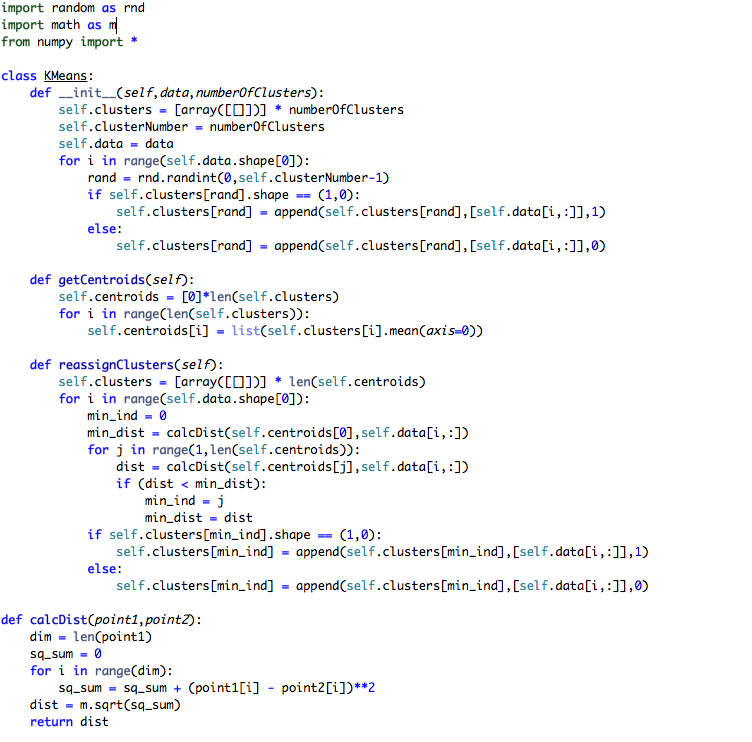
\includegraphics[width=\textwidth]{claudia1.png}
\end{center}

\subsection{K-means Evaluation Module}
As a starting point we look at two criteria to investigate how well the clustering works. The first step is to look at the density of the clusters to see how compacted the clusters are. As a second criteria we will determine the silhouette, which is describing how distant the points in a specific cluster are from the other clusters to investigate the separation of the clusters.

\emph{Functions:}
	\begin{itemize}
		\item Calculate Density 
		\item Silhouette
	\end{itemize}

\subsection{PCA}

Our PCA function takes a matrix and a desired number $n$ of principal components as arguments.  The function generates the covariance matrix for the input matrix and finds the eigenvalues and associated eigenvectors of the covariance matrix.  Lastly, the function generates and returns a projection matrix consisting of the data projected onto the first $n$ principal components.

\subsection{Description of PCA Module}
\emph{PCA Functions:}
\begin{itemize}
	\item Calculate covariance matrix, $S$
	\item Find $M$ largest eigenvalues of $S$
	\item Find eigenvectors corresponding to eigenvalues 
	\item Project data onto eigenvectors
	\item Export Data 
\end{itemize}

\emph{Exceptions:}
\begin{itemize}
	\item Can't compute covariance matrix 
	\item Can't find eigenvalues for covariance matrix
	\item Can't write file 
\end{itemize}

\begin{center}
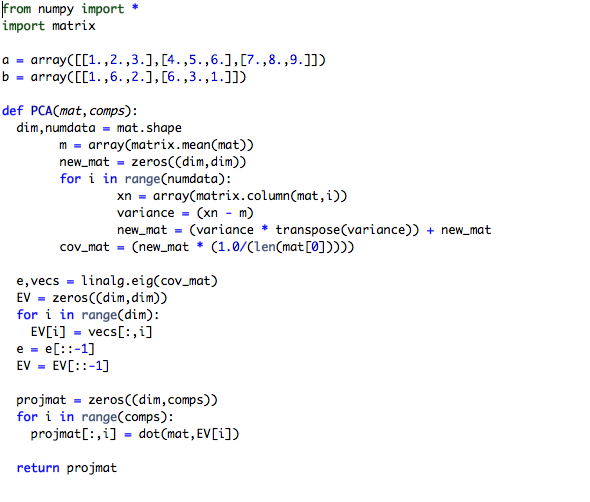
\includegraphics[width=120mm]{claudia5.png}
\end{center}

\subsection{PCA Evaluation Module}
As a preliminary criterion for determining the success of our PCA algorithm, we will look at the variances from projecting the data onto the principal components.
\emph{Functions}
\begin{itemize}
	\item Calculate variances 
\end{itemize}





\section{Timeline}
Today is Sunday, April 8\textsuperscript{th}, 2012. 
There are 3 weeks left. 
\begin{itemize}
	\item First Week: 
		\begin{itemize}
			\item Completely finish rudimentary (but working) versions of k-means clustering and PCA. 
			\item Parse data to format that we want. Currently the datasets are in python pickle format. 
			\item Run our algorithms on actual data. 
			\item Important: identify BEST way to tackle character recognition! Look at different papers to get an idea of 
			what people have found useful in the machine learning community. 
		\end{itemize}

	\item Second Week: 
		\begin{itemize}
			\item Actually implement character recognition 
			\item We have 10,000 training data points. We will train our model, run validation step on 1000 randomly chosen data points (possibly k-fold cross check validation)
			\item After training our model, we will run the algorithm on 1000 data points of the test set.
			\item Look at the results. Plot histogram, implement some other visual approaches to make sure our results are robust. 
		\end{itemize}

	\item Third Week:
		\begin{itemize}
			\item Make sure implementation is free from bugs
			\item Make sure implementation solves the problem for character recognition with responsible probability of success 
			\item Implement GUI and other ``nice'' features on top of the python framework. 
			\item Possibly make it a standalone? 
			\item Look at PyQt
			\item Write up final specs as a README
		\end{itemize}

\end{itemize}



\section{Progress Report}

We have written up rudimentary versions of the k-means and PCA algorithms. 
We have also written up extensive helper functions to read data and plot very basic results. 
We have integrated our code to be used with the following python modules: Python Image Library and 
Numpy. We have set up a git repository and have organized the code in the following manner:

	\begin{itemize}
		\item README.txt - the main README file of the Handwriting Recognition Toolbox.
		\item doc - the draft documents outlining the progress of our work. In particular it contains the latex documents for our drafts. 
		\item data - contains the handwriting data retrieved from online data base. Also contains some randomly generated test data to test the accuracy/robustness of our algorithms. Matrix files parsed as python pickle files for reusability. 
		\item src - contains source code for PCA and k-means. Also has upper-level scripts that handle general implementations such as parsing.
		\item output - contains output files, in text and pickle format. Will also contain plots and other graphical elements in the future. 
	\end{itemize}

Our git repository can be found at 

\begin{center}
\url{https://github.com/friedsam/cs51-final/}
\end{center}

or by cloning at the following address 

\begin{center}
\url{git://github.com/friedsam/cs51-final.git}
\end{center}




\end{document}